\section{1174021 - Muhammad Fahmi}
\subsection{Teori}
\begin{enumerate}

	\item Defenisi Kecerdasan Buatan
	\hfill\break
	Kecerdasan buatan yang jika dalam bahasa inggris ialah Artificial Intelligence (AI) adalah bagian dari ilmu komputer. Dengan penelitian dan pengembangan kecerdasan buatan, ia berusaha untuk tidak hanya berhasil tetapi untuk melengkapi pemikiran manusia dengan program komputer belajar mandiri. AI juga sudah banyak di aplikasikan di dunia bisnis, misalnya, dalam Google Maps. dan Istilah dalam AI juga sudah tidak asing lagi yaitu "Neural Network" dan "Deep learning" yang terkait dengan pengembangan kecerdasan buatan.

	\begin{figure}[H]
	\centering
		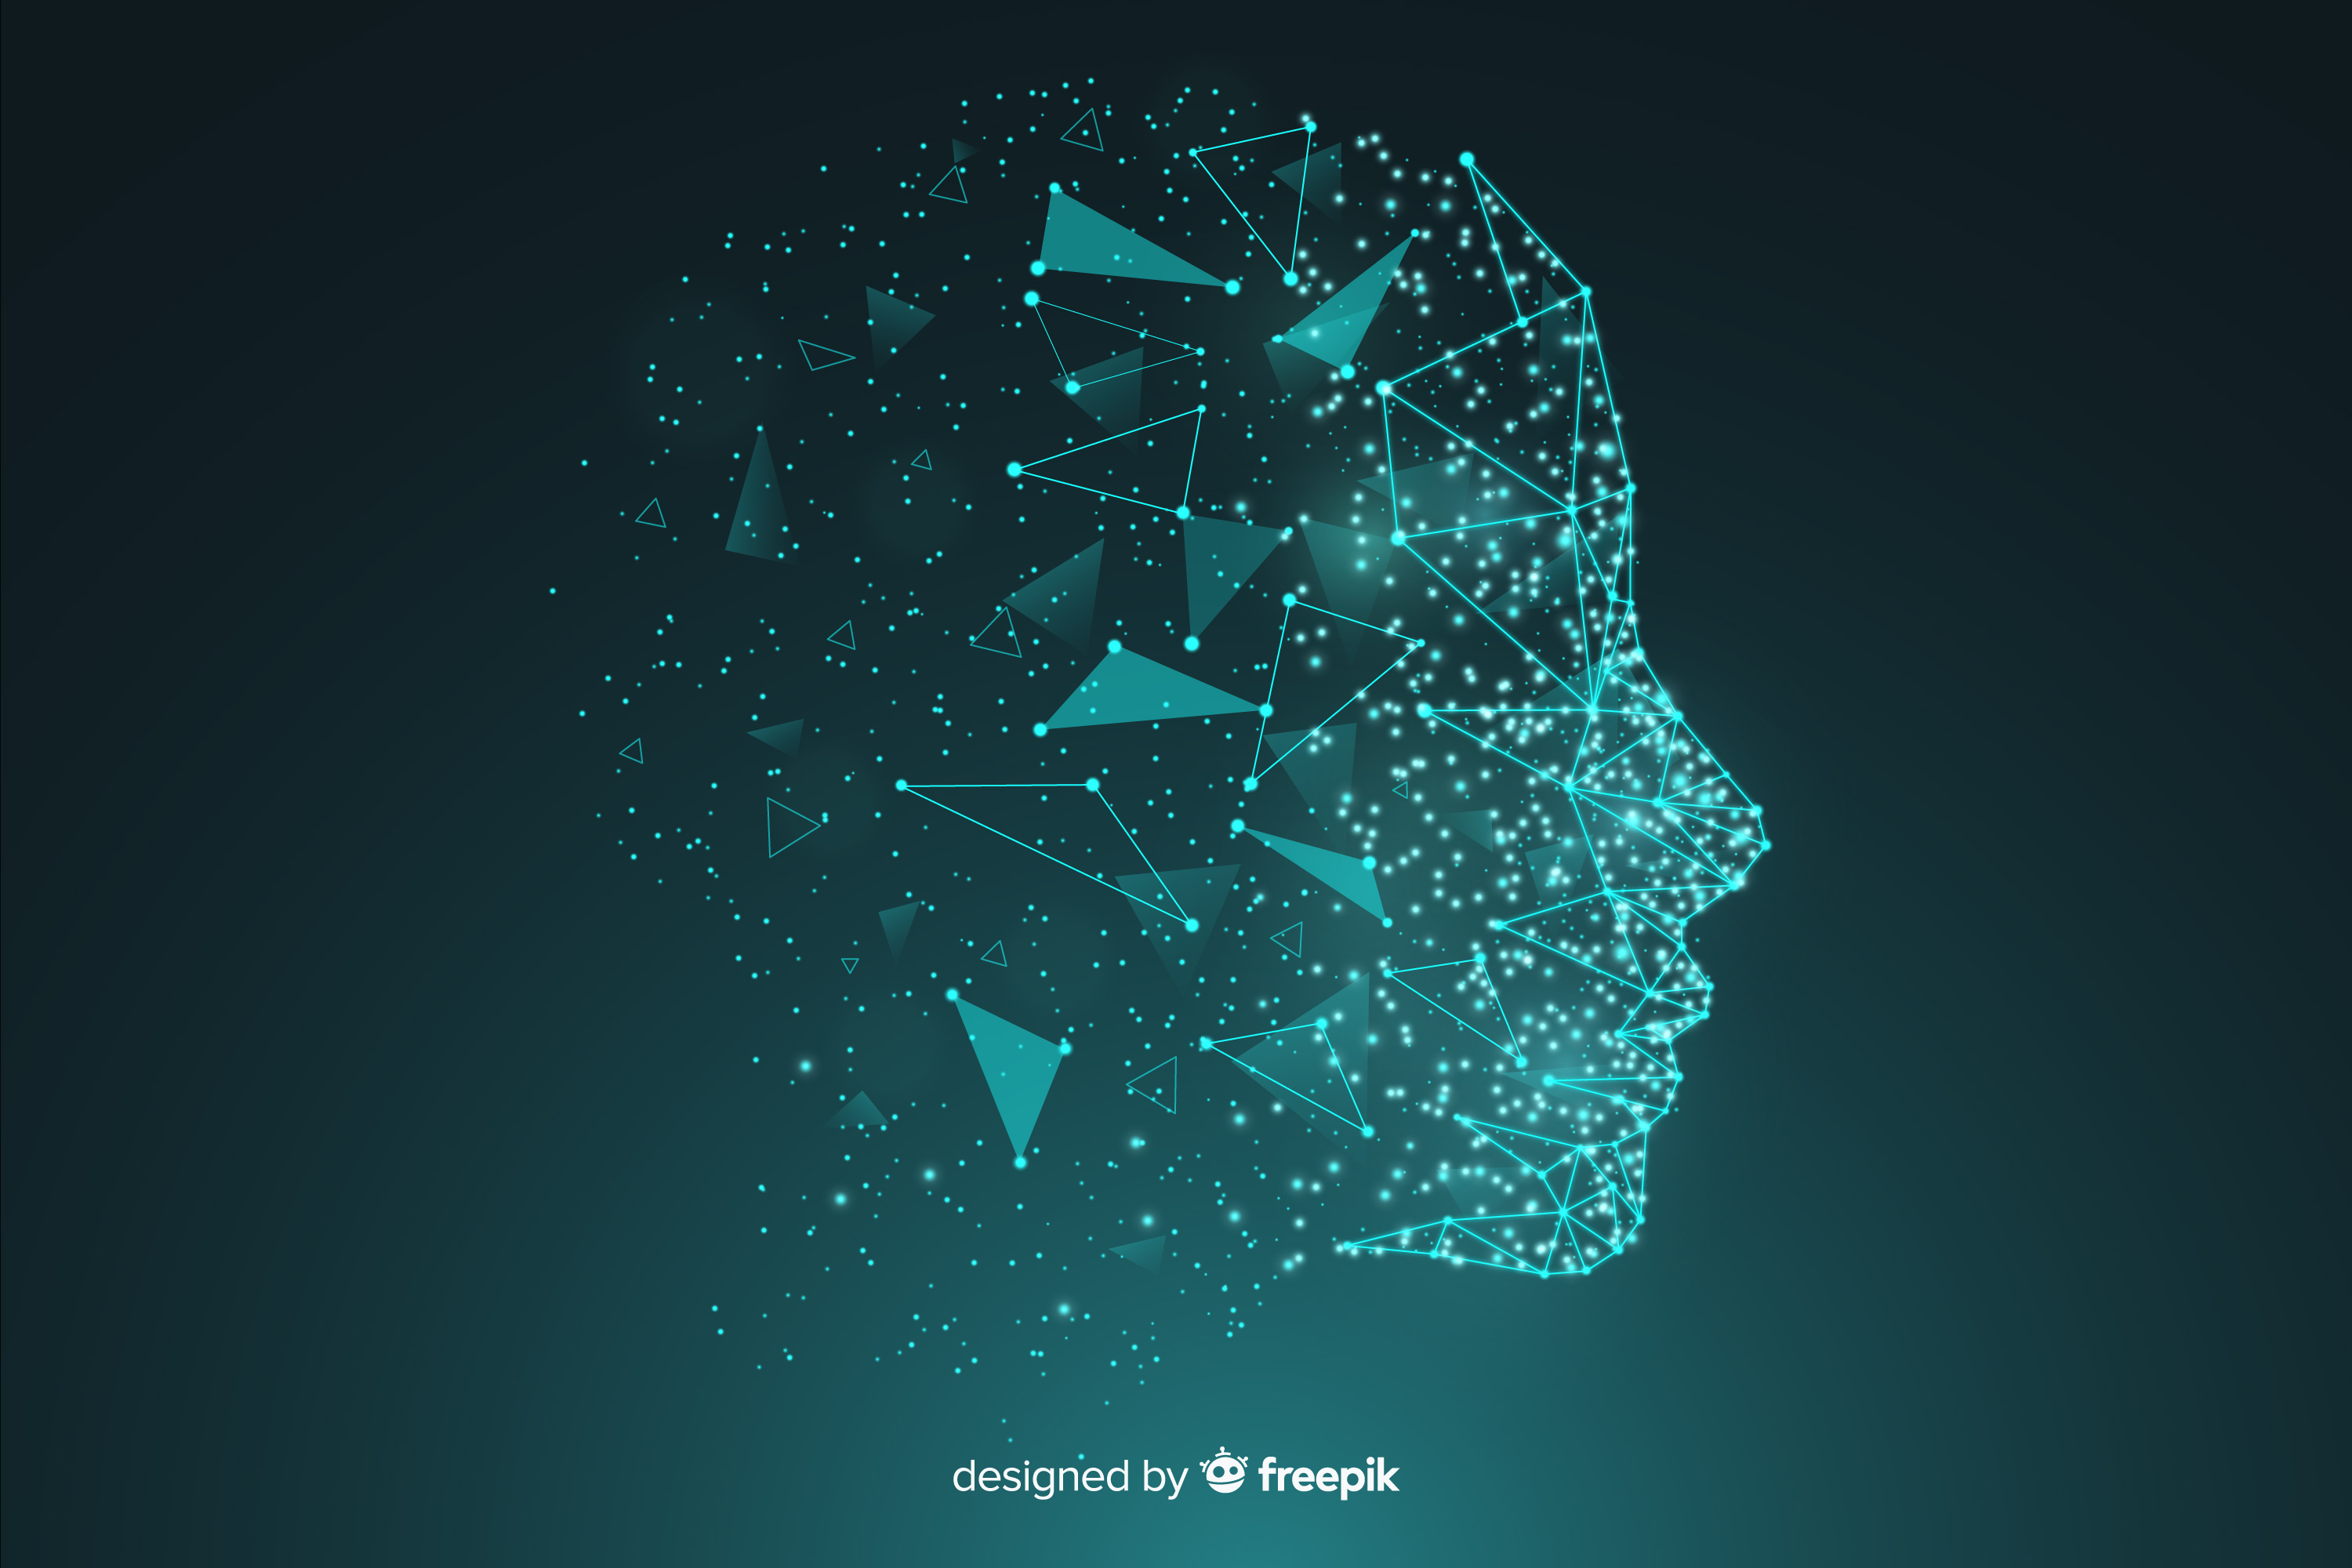
\includegraphics[width=4cm]{figures/1174021/tugas1/materi/1.jpg}
		\caption{Kecerdasan Buatan.}
	\end{figure}

	\item Sejarah dan Perkembangan
	\hfill\break
	Pada tahun 1950 yang bertempat di AS kecerdasan buatan atau AI itu dimulai pada konferensi ilmiah di Dartmouth, M. Minsky, J.McCarthy, A. Newell, dan HA Simon adalah yang pertama berbicara tentang "kecerdasan buatan." Definisi yang sering dikutip untuk kecerdasan buatan diberikan oleh salah satu pendiri subjek, Marvin Minsky, pada tahun 1966: "Kecerdasan Buatan adalah ilmu membuat mesin melakukan hal-hal yang membutuhkan kecerdasan jika dilakukan oleh manusia." Jadi, ditentukan bahwa kecerdasan buatan adalah ilmu dan kedua mesin dapat mengambil alih pekerjaan manusia yang membutuhkan kecerdasan manusia. Adapun mengapa AI yaitu untuk pemecah an masalah umum dari para peneliti Newell, Shaw, dan Simon pada tahun 1960-an. Penelitian ini dapat memecahkan masalah sederhana. Namun, hasil penelitian tersebut tidak dapat digeneralisasi. Pada akhir 1960-an, program lain ditulis dengan ELIZA. Dengan demikian, Joseph Weizenbaum, seorang peneliti MIT,simulasikan sesi terapi. Pada tahun-tahun berikutnya, sains muda terus dikembangkan, yang diproduksi oleh MYCIN pada awal 1970-an dalam sistem inovatif lain berbasis AI. MYCIN dapat membantu dokter mendiagnosis.
	

	\item Kecerdasan buatan terbagi atas beberapa metode yaitu:
	\hfill\break
	Supervised learning, Unsupervised Learning, Klasifikasi, Regresi, Dataset, Trainingset dan juga Testingset.
	\begin{itemize}
		\item Supervised Learning
		\hfill\break
		Sebuah algoritma pembelajaran mesin yang dapat menerapkan informasi yang sudah ada dalam data dengan memberikan label tertentu, misalnya data yang telah diklasifikasikan sebelumnya (diarahkan). Algoritma ini mampu memberikan target untuk output yang dilakukan dengan membandingkan pengalaman belajar masa yang sudah lampau.
		\item Unsupervised Learning 
		\hfill\break
		Berbeda dengan Supervised Learning, Unsupervised Learning ialah sebuah pembelajaran mesin tanpa pengawasan adalah pembelajaran mesin yang digunakan pada data yang tidak memiliki informasi yang dapat diterapkan secara langsung (tidak diarahkan). Algoritma ini diharapkan dapat menemukan struktur tersembunyi dalam data yang tidak berlabel.
		\item Klasifikasi
		\hfill\break
		Klasifikasi adalah sampel milik dua kelas atau lebih dan ingin belajar dari data yang sudah diberi label cara memprediksi kelas data yang tidak berlabel. Contoh masalah klasifikasi adalah pengenalan digit tulisan tangan, di mana tujuannya adalah untuk menetapkan masing-masing vektor input ke salah satu dari sejumlah kategori diskrit. 
		\item Regresi
		\hfill\break
		Regrasi ialah sebuah metode untuk mengembangkan model (persamaan) yang menjelaskan hubungan antara beberapa variabel. Output dari analisis regresi adalah persamaan regresi. Dalam model regresi variabel dibagi menjadi dua bagian, yaitu variabel respon atau yang biasa juga disebut variabel dependen dan variabel explanatory atau juga biasa disebut variabel prediktor atau disebut juga variabel independen.
		\item Data set
		\hfill\break
		Dataset adalah sebuah kumpulan data atau objek dan bagaimana relasi dalam memori. Struktur Dataset mirip dengan data di dalam database. Dataset berisi koleksi dari datatable maupun data relasi.
		\item Training Set
		\hfill\break
		Training set ialah bagian dari dataset yang berfungsi untuk membuat prediksi atau mengatur fungsi dari algoritma-algoritma yang ada. Fungsi nya yang lain juga ada sesuai tujuannya masing-masing. Trainingset memberikan instruksi melalui algoritma sehingga mesin dapat mengerti dan membuat kolerasi sendiri.		
		\item Testing Set
		\hfill\break
		Sama seperti training set, testing set juga bagian dari dataset yang berfungsi menguji untuk melihat akurasinya, atau bisa juga untuk melihat suatu kinerja atau performa.
	\end{itemize}
\end{enumerate}
\subsection{Praktek}
\begin{enumerate}
	\item Instalasi Library scikit dari Anaconda, mencoba kompilasi dan uji coba ambil contoh kode dan lihat variabel explorer
	\hfill\break
	\begin{figure}[H]
		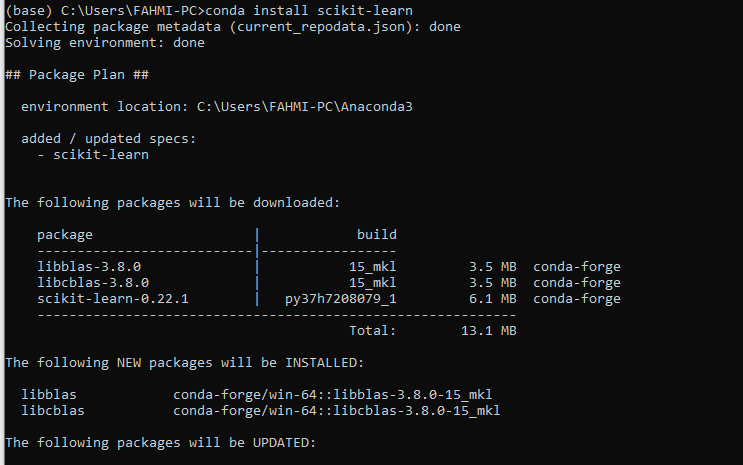
\includegraphics[width=4cm]{figures/1174021/tugas1/materi/2.PNG}
		\centering
		\caption{Instalasi Library Scikit Learn}
	\end{figure}
	\begin{figure}[H]
		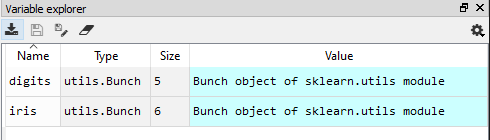
\includegraphics[width=4cm]{figures/1174021/tugas1/materi/3.PNG}
		\centering
		\caption{Isi Variabel Explorer}
	\end{figure}
	\item Uji coba loading an example dataset
	\hfill\break
	\lstinputlisting[firstline=10, lastline=14]{src/1174021/tugas1.py}
	\item Uji coba Learning dan predicting
	\hfill\break
	\lstinputlisting[firstline=18, lastline=21]{src/1174021/tugas1.py}
	\item Uji coba Model Persistence
	\hfill\break
	\lstinputlisting[firstline=25, lastline=41]{src/1174021/tugas1.py}
	\item Uji coba Conventions
	\hfill\break
	\lstinputlisting[firstline=44, lastline=56]{src/1174021/tugas1.py}
\end{enumerate}
\subsection{Penanganan Error}
\begin{enumerate}
	\item ScreenShoot Error
	\begin{figure}[H]
		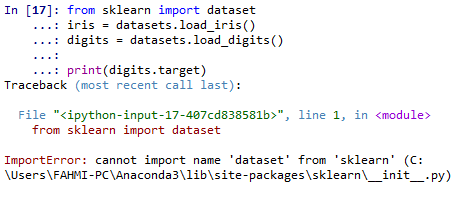
\includegraphics[width=4cm]{figures/1174021/tugas1/error/1.PNG}
		\centering
		\caption{Import Error}
	\end{figure}
	\begin{figure}[H]
		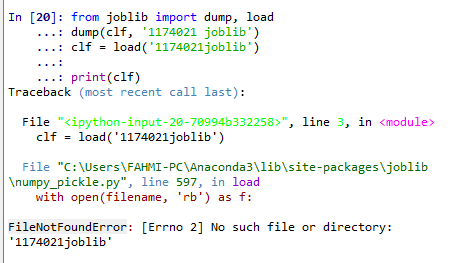
\includegraphics[width=4cm]{figures/1174021/tugas1/error/2.PNG}
		\centering
		\caption{FileNotFoundError}
	\end{figure}
	\item Tuliskan Kode Error dan Jenis Error
	\begin{itemize}
		\item Import Error
		\item FileNotFoundError
	\end{itemize}
	\item Cara Penangan Error
	\begin{itemize}
		\item Import Error
		\hfill\break
		Error terdapat typo pada dataset, seharusnya datasets
		\item FileNotFoundError
		\hfill\break
		Error terdapat pada 1174021joblib, tidak ada file yang dibaca, seharusnya 1174021.joblib
	\end{itemize}
\end{enumerate}
\subsection{Bukti Tidak Plagiat}
\begin{figure}[H]
	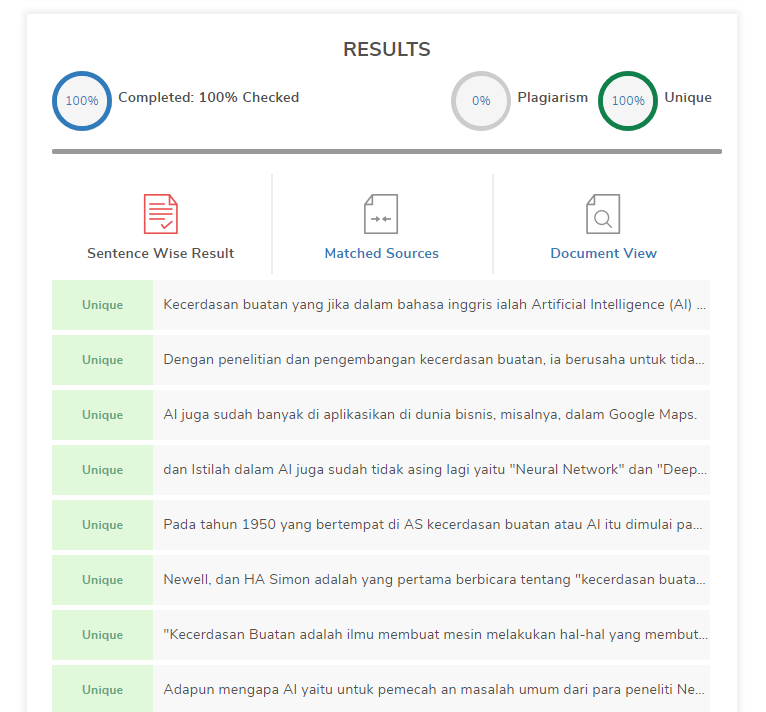
\includegraphics[width=4cm]{figures/1174021/tugas1/buktiplagiat/1.PNG}
	\centering
	\caption{Bukti Tidak Melakukan Plagiat Chapter 1}
\end{figure}